%! Author = danielmendes
%! Date = 29.11.24

\chapter{Optimierungen von Datentypen}\label{ch:data-types}

Das erste Thema in Bezug auf die Performance-Optimierung von Datenbanken sind die unterschiedlichen Datentypen und deren Auswirkungen auf die Performance.
Bei der Auswahl des korrekten Datentyps gibt es unterschiedliche Faktoren, die vom jeweiligen Typen abhängen.
Besonders werden die unterschiedlichen Implementierungen von numerischen und zeichenkettenbasierten Datentypen analysiert.
Am Ende des Kapitels werden die Ergebnisse der Benchmarks betrachtet.
Zunächst wird aber mit den allgemeineren Prinzipien begonnen.

\section{Allgemeine Faktoren}\label{sec:data-types-allgemeine-faktoren}

In diesem Abschnitt werden die geltenden Grundsätze behandelt, die generell bei der Wahl der Datentypen beachtet werden sollten.
Bevor das behandelt wird, muss geklärt werden, welche Schritte zur Auswahl von Datentypen durchgeführt werden (\cite[S. 115--145]{schwartz2012high}).
Als erstes wird die übergeordnete Kategorie des Datentyps, wie beispielsweise numerisch, textbasiert oder zeitbezogen, festgelegt.
Anschließend sollte der spezifische Typ ausgewählt werden.
Für numerische Daten kommen beispielsweise Ganzzahlen wie \texttt{INT} oder Fließkommazahlen wie \texttt{FLOAT} und \texttt{DOUBLE} infrage.
Die spezifischen Typen können dieselbe Art von Daten speichern, unterscheiden sich jedoch im Bereich der Werte, die sie speichern können.
Auch sind sie unterschiedlich in der Genauigkeit (engl.\ Precision), die sie erlauben und dem physischen Speicherplatz, den sie entweder auf der Festplatte oder im Arbeitsspeicher benötigen.
Einige Datentypen haben auch spezielle Verhaltensweisen und Eigenschaften.

Der erste Grundsatz für Datentypen besagt, dass kleiner besser ist.
Deshalb sollte man den kleinstmöglichen Datentypen wählen, den man speichern kann und der die vorhandenen Daten entsprechend repräsentieren kann.
Dadurch wird weniger Speicherplatz im Arbeitsspeicher und CPU-Cache benötigt, was wiederum zu schnelleren Abfragen führt.
Außerdem ist bei der Benutzung des kleinstmöglichen Typs eine einfache Typveränderung möglich.
Wenn die vorhandenen Daten beispielsweise falsch eingeschätzt wurden, lässt sich der Typ nachträglich mit wenig Aufwand in einen größeren umwandeln.

Eine weitere allgemeine Richtlinie ist die Einfachheit von Datentypen.
So sind Integer-Werte beispielsweise leichter zu verarbeiten als Character.
Daher sollte man stets einen Integer wählen, wenn er die Daten korrekt abbilden kann.
Begründen kann es damit, dass für einfachere Datentypen weniger CPU-Zyklen benötigt werden, um Operationen auszuführen.
Im Fall von Integer und Character liegt der Unterschied in den Character Sets und Sortierregeln, die den Vergleich von Character erschweren.

Die letzte Regel zur Performanceverbesserung ist die Vermeidung von \texttt{NULL}.
Viele Tabellen enthalten \texttt{NULLABLE}-Spalten, obwohl keine \texttt{NULL}-Werte gespeichert werden müssen, da \texttt{NULL} die Standardeinstellung ist.
Daher sollten solche Spalten bei der Tabellenerstellung mit dem Identifier \texttt{NOT NULL} definiert werden, es sei denn, \texttt{NULL}-Werte sind erforderlich.

\begin{quote}
    \enquote{A missing NOT NULL constraint can prevent index usage in an Oracle database-especially for count(*) queries.} (\cite[S. 57]{winand2011sql})
\end{quote}

Mit \texttt{NULL} wird es auch für MySQL schwieriger, Abfragen zu optimieren, da Indizes und Wertevergleiche mehr Speicherplatz benötigen.
Dies liegt daran, dass indizierte nullable Spalten ein zusätzliches Byte pro Eintrag erfordern, wodurch ein Index mit fester Größe in einen variablen umgewandelt wird.
Der Leistungsunterschied zwischen \texttt{NULL} und \texttt{NOT NULL} ist zwar gering, kann jedoch, besonders in Verbindung mit Indizes, spürbar sein.

Abschließend ist darauf hinzuweisen, dass MySQL eine Vielzahl von Aliasen für Datentypen unterstützt, darunter \texttt{INTEGER}, \texttt{BOOL} und \texttt{NUMERIC}.
Obwohl diese Aliase potenziell zu Verwirrung führen können, haben sie keinen Einfluss auf die Performance.
Im Wesentlichen funktioniert es so, dass ein aliasierter Datentyp beim Erstellen einer Tabelle intern in den Basistyp umgewandelt wird.
Dies lässt sich mit dem Befehl \texttt{SHOW CREATE TABLE} bestätigen.

\section{Funktionsweise individueller Datentypen}\label{sec:data-types-verhaltensweise-einzelner-datentypen}

Der erste Datentyp, bei dem das Verhalten genauer betrachtet wird, ist der numerische Datentyp.
Bei diesem kann zwischen Ganzzahlen und Fließkommazahlen gewählt werden.
Die spezifischen Typen unterscheiden sich nur in der Anzahl der Bits, die sie speichern können.
\texttt{SMALLINT} kann 16 Bits speichern, während \texttt{INT} 32 und \texttt{BIGINT} 64 Bits speichern kann (\cite{mysql_data_types_numeric}).
Dementsprechend verändert sich auch der mögliche Wertebereich der Zahlen, die durch den Speicherplatz abgedeckt sind.
Mit den optionalen \texttt{UNSIGNED}-Attributen können keine negativen Werte gespeichert werden können.
Dafür verdoppelt sich die obere Grenze der positiven Werte, während der Speicherplatz und die Leistung unverändert bleiben.
Die Berechnung des Wertebereichs für \texttt{SIGNED} und \texttt{UNSIGNED} erfolgt nach den folgenden Formeln:

\vspace{-27pt}
\begin{gather}
    \text{Signed: } -2^{(N-1)} \text{ bis } 2^{(N-1)} - 1\label{eq:equation-signed} \\
    \text{Unsigned: } 0 \text{ bis } 2^N - 1\label{eq:equation-unsigned}
\end{gather}

\vspace{-10pt}
\textbf{Hinweis:} $N$ entspricht der Anzahl der Bits.

Wenn die Wertebereiche für den Datentyp \texttt{TINYINT} in MySQL berechnet werden sollen, muss für $N$ der Wert 8 eingesetzt werden.
Als Ergebnis ergeben sich für \texttt{SIGNED} die Werte von -128 bis 127 und für \texttt{UNSIGNED} die Werte von 0 bis 255.
Bei einem Beispiel mit 150 Werten kann anstelle von \texttt{SMALLINT} also einfach \texttt{UNSIGNED} verwendet werden, um Speicherplatz zu sparen.

Eine Breitenangabe wie \texttt{INT(11)} beeinflusst nur die Anzeige und nicht den Wertebereich oder die Speicheranforderungen.
Um dies zu beweisen, wird die folgende Tabelle erstellt:

\lstinputlisting[
    language=sql,
    style=custom_daniel,
]{Scripts/Data_Types/01_testint_create.sql}
\vspace{-7pt}

Für beide Spalten wurde der Datentyp \texttt{INT} gewählt und da überprüft werden soll, ob die Breitenangabe einen Einfluss auf die Speicheranforderungen hat, wird versucht, die Grenzen von \texttt{INT} einzufügen.
Da \texttt{INT} 32 Bits benötigt, ergeben sich folgende Grenzen: $2^{(32-1)} - 1 = 2147483647$ und $-2^{(32-1)} = -2147483648$.

\vspace{-7pt}
\lstinputlisting[
    language=sql,
    caption=Inserts und Selects für Testtabelle,
    label={lst:data-types-testint_queries_sql},
    style=custom_daniel,
]{Scripts/Data_Types/02_testint_queries.sql}
\vspace{-9pt}
\begin{table}[H]
    \centering
    \caption{Ergebnis der SQL-Abfrage aus \ref{lst:data-types-testint_queries_sql}}
    \vspace{-3pt}
    \begin{tabular}{l|c|c}
        & \textbf{int\_5} & \textbf{int\_11} \\ \hline
        \textbf{obere Grenze} & 2147483647 & 2147483647 \\ \hline
        \textbf{untere Grenze} & -2147483648 & -2147483648
    \end{tabular}
    \label{tab:int_values}
\end{table}
\vspace{-9pt}

Bei der Ausführung der Insert-Befehle wird keine Fehlermeldung angezeigt, weshalb \texttt{INT(5)} und \texttt{INT(11)} beide die Grenzwerte speichern können.
Damit wurde gezeigt, dass die Breitenangabe keinen Einfluss auf die Speicheranforderungen hat, sondern lediglich die Anzeige beeinflusst.

Neben dem Typ für Ganzzahlen gibt es auch den Typ für Festkommazahlen, der in MySQL als \texttt{DECIMAL} bezeichnet wird.
Eine Festkommazahl ist eine Zahl mit einem festen Dezimalpunkt, bei der sowohl die Anzahl der Dezimalstellen als auch die maximale Anzahl der Ziffern vor und nach dem Dezimalpunkt definiert sind.
Damit ist er auch für die Speicherung von Ganzzahlen geeignet.
\texttt{DECIMAL(18, 9)} beispielsweise speichert neun Ziffern vor und nach dem Dezimalpunkt und benötigt dafür 9 Bytes Speicherplatz.
Zudem speichert \texttt{DECIMAL} die Zahlen in einer binären Zeichenkette mit neun Ziffern pro vier Bytes und unterstützt insgesamt bis zu 65 Ziffern.

Ein weiterer numerischer Datentyp sind die Fließkommazahlen, zu denen \texttt{FLOAT} und \texttt{DOUBLE} gehören.
Fließkommazahlen verwenden die Gleitkomma-Arithmetik und sind für ungefähre Berechnungen optimiert.
\texttt{FLOAT} benötigt 4 Bytes, während \texttt{DOUBLE} 8 Bytes Speicherplatz beansprucht und eine höhere Präzision sowie einen größeren Wertebereich bietet.
Die Gleitkomma-Arithmetik ist aufgrund der nativen Verarbeitung durch die CPU deutlich schneller als die präzise Berechnung mit \texttt{DECIMAL}, bringt jedoch einen gewissen Präzisionsverlust mit sich.
Alternativ kann man auch \texttt{BIGINT} nutzen, um sowohl die Ungenauigkeit von Gleitkomma-Speicherungen als auch die höheren Kosten der \texttt{DECIMAL}-Arithmetik zu vermeiden.

Als Nächstes werden die zeichenkettenbasierten Datentypen betrachtet.
Die beiden Haupttypen sind \texttt{VARCHAR} und \texttt{CHAR}.
\texttt{VARCHAR} speichert die Zeichenfolgen mit variabler Länge und benötigt daher weniger Speicherplatz als Typen mit fester Länge, da nur so viel Platz verwendet wird, wie tatsächlich benötigt wird.
Zusätzlich werden ein oder zwei Bytes für die Speicherung der Länge der Zeichenfolge verwendet (1 Byte für < 255 Bytes Zeichenfolge).
Durch diese effiziente Speichernutzung ist \texttt{VARCHAR} der am häufigsten verwendete Datentyp für Zeichenketten.
Es gibt jedoch auch Nachteile, da Aktualisierungen der Werte zu wachsenden Zeilen führen und damit auch zu zusätzlicher Verarbeitung der Speicher-Engine.
Interessant ist auch, dass die Speicherung von \texttt{hello} in \texttt{VARCHAR(5)} oder \texttt{VARCHAR(200)} zwar gleich viel Speicherplatz benötigt, jedoch ineffizienter bei Sortierungen oder Operationen auf temporären Tabellen sein kann.
Deshalb sollte immer so viel Platz reserviert werden, wie tatsächlich benötigt wird.

Im Gegensatz zu \texttt{VARCHAR} hat \texttt{CHAR} hingegen eine feste Länge und MySQL reserviert auch den nicht gebrauchten Platz für die angegebene Anzahl an Zeichen.
Daher ist \texttt{CHAR} ideal für sehr kurze Strings oder Werte, die alle nahezu gleich lang sind, da \texttt{VARCHAR(1)} aufgrund des Längen-Bytes 2 Bytes benötigt, \texttt{CHAR(1)} hingegen nur 1 Byte.
Außerdem bleibt die Speicherstruktur bei Aktualisierungen von \texttt{CHAR} unverändert, weshalb er besser geeignet ist, wenn die Daten häufig geändert werden.
Dafür ist \texttt{CHAR} nicht dafür geeignet, wenn die maximale Spaltenlänge deutlich größer ist als die durchschnittliche Wertelänge.

Als Letztes werden die zeitbezogenen Datentypen \texttt{DATE}, \texttt{TIME}, \texttt{TIMESTAMP} und \texttt{DATETIME} behandelt.
Der Datentyp \texttt{DATE} speichert nur das Datum ohne Uhrzeit und ist besonders speichereffizient, während \texttt{TIME} ausschließlich eine Uhrzeit oder Zeitspanne, auch über 24 Stunden hinaus, erfasst.
Die anderen beiden speichern das Datum mit Uhrzeit und haben eine Genauigkeit von einer Sekunde.
\texttt{TIMESTAMP} benötigt nur halb so viel Speicherplatz wie \texttt{DATETIME} und ist zeitzonenbewusst, hat aber dafür einen deutlich kleineren Wertebereich.
Abhängig von der Information, die gespeichert werden soll, wählt man den passenden zeitbezogenen Datentyp.

\section{Analyse der Benchmarks}\label{sec:data-types-analyse-der-benchmarks}

Der erste Leitsatz, der untersucht wird, besagt, dass Spalten nach Möglichkeit als \texttt{NOT NULL} deklariert werden sollten.
Zum Nachweis wird die Kundentabelle aus~\ref{lst:tools-create-table-kunde} verwendet, bei der einmal alle Spalten als \texttt{NOT NULL} deklariert sind und einmal der Standardwert genutzt wird.
Wenn das Attribut nicht deklariert wird, können NULL-Werte in die Tabelle eingefügt werden.
Um bei Select-Abfragen mit \texttt{WHERE}-Klauseln sowie \texttt{COUNT}- und \texttt{GROUP BY}-Befehlen die gleiche Anzahl an Zeilen zu erhalten, werden NULL-Werte beim Einfügen ausgeschlossen.

In der Grafik~\ref{data-types-null-reads} sind die Ergebnisse der Select-Befehle zu sehen, wobei die Werte für \texttt{NOT NULL} im Durchschnitt höher sind als für \texttt{WITH NULL}.
Höhere Werte bedeuten mehr Abfragen pro Sekunde und deuten auf bessere Performance hin, weshalb man sagen kann, dass \texttt{NOT NULL} besser performt als \texttt{WITH NULL}.
Wenn man auf die y-Achse schaut, fällt aber auf, dass die Werte nicht so weit auseinanderliegen und damit sind die Unterschiede sehr gering.
Daher sollte die Entscheidung, eine Spalte als \texttt{NOT NULL} zu deklarieren, vor allem aus Gründen der Datenintegrität und -konsistenz und nicht aus Performancegründen getroffen werden.

\vspace{-8pt}
\begin{figure}[H]
    \centering
    \begin{subfigure}[t]{0.48\textwidth}
        \centering
        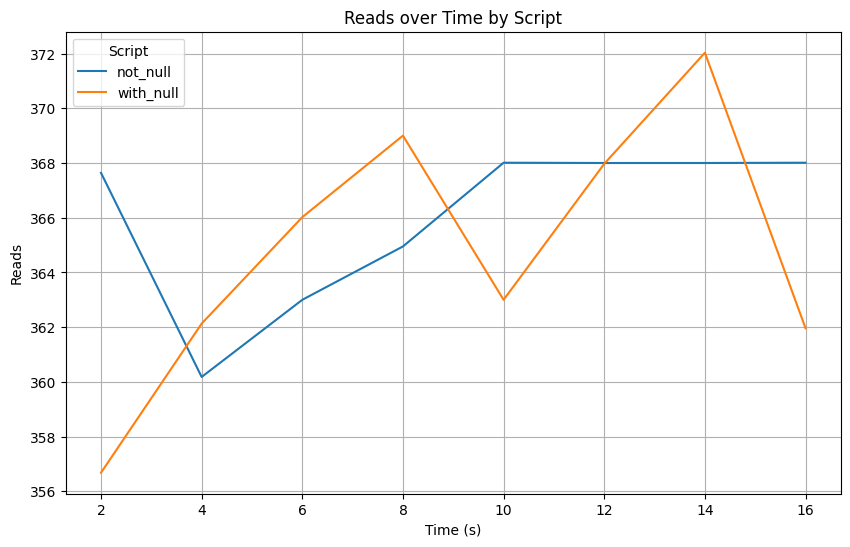
\includegraphics[width=\textwidth]{PNGs/Script/Data_Types/Null/null-check/Reads}
        \caption{Vergleich von NULL und NOT NULL}
        \label{data-types-null-reads}
    \end{subfigure}
    \hfill
    \begin{subfigure}[t]{0.48\textwidth}
        \centering
        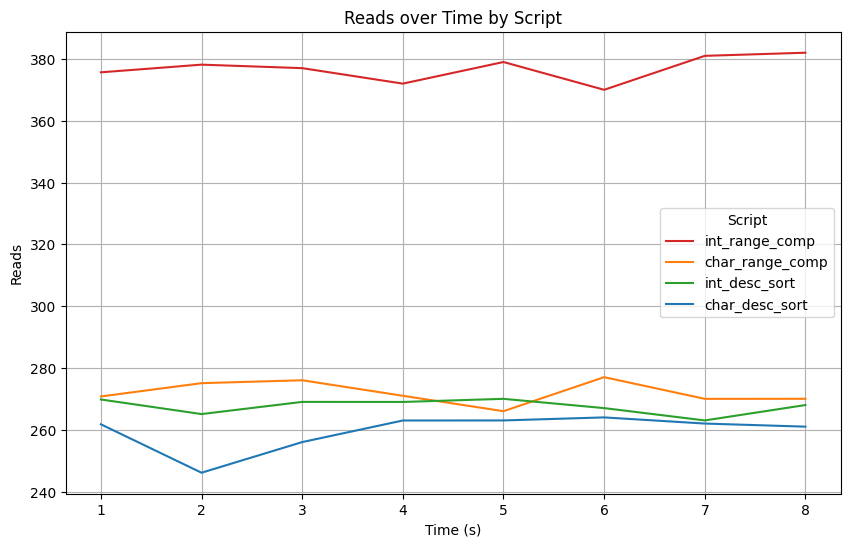
\includegraphics[width=\textwidth]{PNGs/Script/Data_Types/Simpler/int-char/Reads}
        \caption{Vergleich von INT und CHAR}
        \label{data-types-int-char-reads}
    \end{subfigure}
    \vspace{-6pt}
    \caption[Datentypen: Vergleich mit Not Null, sowie Int und Char]{Vergleich von \texttt{NULL} und \texttt{NOT NULL}, sowie \texttt{INT} und \texttt{CHAR}}
\end{figure}
\vspace{-20pt}

Um zu zeigen, dass bei der Wahl zwischen unterschiedlichen Datentypen der einfachere bevorzugt werden sollte, wird erneut die Kundentabelle verwendet.
Für diesen Benchmark wird jeweils der Datentyp des Schlüsselattributs der Tabelle geändert.
Zunächst wird eine Kundentabelle mit einem \texttt{INT}-Primärschlüssel erstellt, gefolgt von einer weiteren mit \texttt{CHAR}.
Die Performance der Schreibbefehle ist in beiden Fällen etwa gleich.
Bei den Lesebefehlen sieht das anders aus (siehe~\ref{data-types-int-char-reads}).
Wenn man einen Wertebereich abfragt, dann ist \texttt{INT} deutlich schneller (etwa 20\%) als \texttt{CHAR}.
Bei der Sortierung hat \texttt{INT} ebenfalls einen Vorteil, jedoch fallen die Abstände deutlich geringer aus.

Als letztes soll der Vergleich unterschiedlicher Datentypen erfolgen.
Hierfür wird die gleiche Tabelle wie beim Vergleich von \texttt{INT} und \texttt{CHAR} verwendet, jedoch werden diesmal verschiedene numerische oder zeichenkettenbasierte Typen als Primärschlüssel eingesetzt.
Beim Vergleich der numerischen Typen zeigt sich, dass \texttt{DECIMAL} mit deutlichem Abstand am langsamsten ist (Abbildung~\ref{data-types-smaller-number-type-reads}).
Danach folgt, wie vermutet, der nächstgrößere Datentyp \texttt{BIGINT}.
Das lässt sich sowohl an der Grafik als auch an der Legende erkennen, die die Typen nach Performance absteigend sortiert.
Die Legende hilft vor allem deswegen, weil die unterschiedlichen Werte auch aufgrund der Skalierung der y-Achse sehr stark schwanken.
Als Nächstes kommen \texttt{INT}, \texttt{MEDIUMINT} und \texttt{SMALLINT}, wobei die Unterschiede kleiner sind als erwartet.
Dies wird vermutlich darauf zurückzuführen sein, dass die Abfragen nur auf einer Tabelle mit wenigen tausend Datensätzen ausgeführt wurden.
In der Praxis mit Millionen von Datensätzen dürften die Unterschiede zwischen den Typen größer sein als in diesem Vergleich.

\vspace{-12pt}
\begin{figure}[H]
    \centering
    \begin{subfigure}[t]{0.48\textwidth}
        \centering
        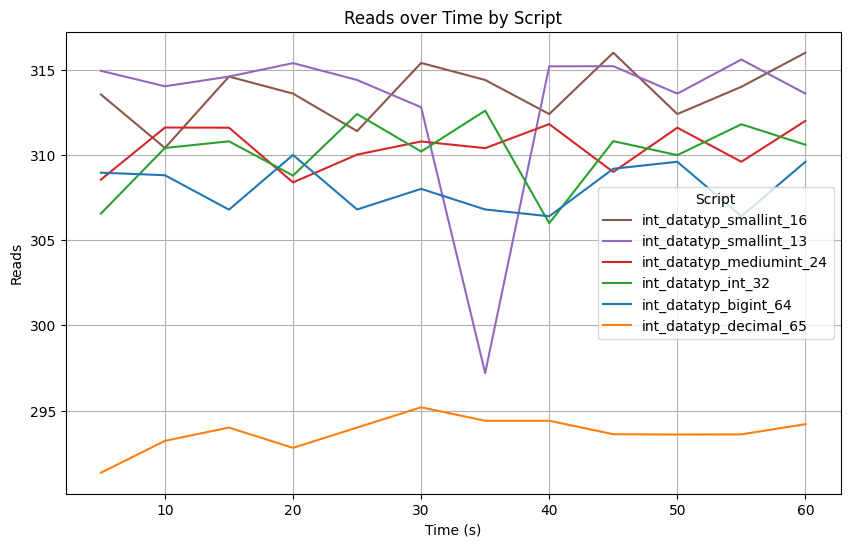
\includegraphics[width=\textwidth]{PNGs/Script/Data_Types/Smaller/number-type/Reads}
    \end{subfigure}
    \vspace{-10pt}
    \caption[Datentypen: Numerische Datentypen]{Vergleich von unterschiedlichen zeichenkettenbasierten Typen}
    \label{data-types-smaller-number-type-reads}
\end{figure}
\vspace{-20pt}

Beim Vergleich zwischen den beiden Zeichenketten-Typen \texttt{CHAR} und \texttt{VARCHAR} ist unabhängig von der Länge zu erkennen, dass \texttt{VARCHAR} effizienter ist als \texttt{CHAR} (siehe~\ref{fig:data-types-smaller-string-type-reads}).
Im ersten Vergleich wurde jeweils eine Länge von 4 Stellen verwendet und beim zweiten Vergleich eine Länge von 64 Stellen.
Bei beiden untersuchten Längen ist \texttt{VARCHAR} schneller als \texttt{CHAR}.

Als letzten Vergleich wurden beide Zeichenketten-Typen mit der Länge von 255 Stellen definiert, aber mit unterschiedlich vielen Stellen befüllt.
Anschließend wurden bei beiden Tabellen die Werte aktualisiert, wobei in der Namen-Spalte zufällig einige Stellen hinzugefügt wurden.
Dabei war \texttt{CHAR} schneller als \texttt{VARCHAR} (\ref{fig:data-types-smaller-string-type-length-writes}).
Dies bestätigt die Vermutungen aus Abschnitt~\ref{sec:data-types-verhaltensweise-einzelner-datentypen}, da die Vorteile von \texttt{CHAR} insbesondere bei der Aktualisierung von Werten zum Tragen kommen, während \texttt{VARCHAR} bei der Selektion von Werten besser abschneidet.

\vspace{-10pt}
\begin{figure}[H]
    \centering
    \begin{subfigure}[t]{0.48\textwidth}
        \centering
        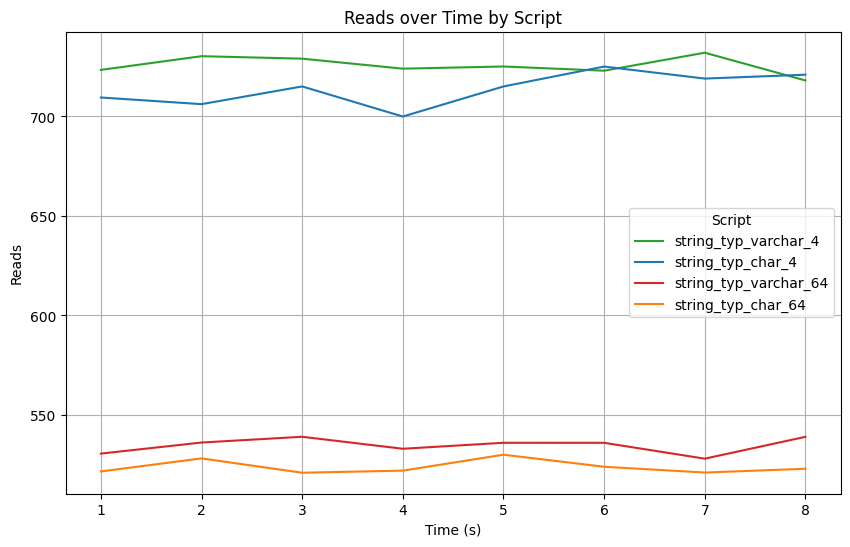
\includegraphics[width=\textwidth]{PNGs/Script/Data_Types/Smaller/string-type/Reads}
        \caption{Unterschiedliche Zeichenketten-Typen}
        \label{fig:data-types-smaller-string-type-reads}
    \end{subfigure}
    \hfill
    \begin{subfigure}[t]{0.48\textwidth}
        \centering
        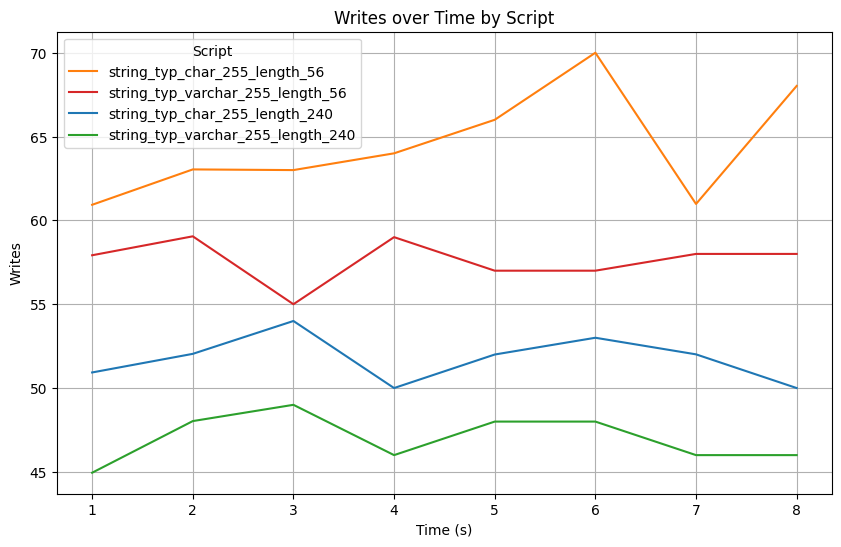
\includegraphics[width=\textwidth]{PNGs/Script/Data_Types/Smaller/string-type-length/Writes}
        \caption{Bei unterschiedlichem Befüllungsgrad}
        \label{fig:data-types-smaller-string-type-length-writes}
    \end{subfigure}
    \vspace{-6pt}
    \caption[Datentypen: Zeichenkettenbasierte Typen]{Vergleich von unterschiedlichen zeichenkettenbasierten Typen}
\end{figure}